\chapter{Architecture}\label{ch:arch}

The application is compound by three components:
\begin{enumerate*}[label=(\roman*)]
	\item The scraper, which can be active or not, that uses online
		exchanges API to download market data and save it in a document
		database in a common structure, even if data comes from multiple
		sources;
	\item The server, which accepts requests from the client and runs the
		strategies over the data saved in the database, then it responds
		with the results;
	\item The client, \idest*{the front-end application used by the users to
		submit strategies to the server and get back the results}.
\end{enumerate*}

\begin{figure}[p]
	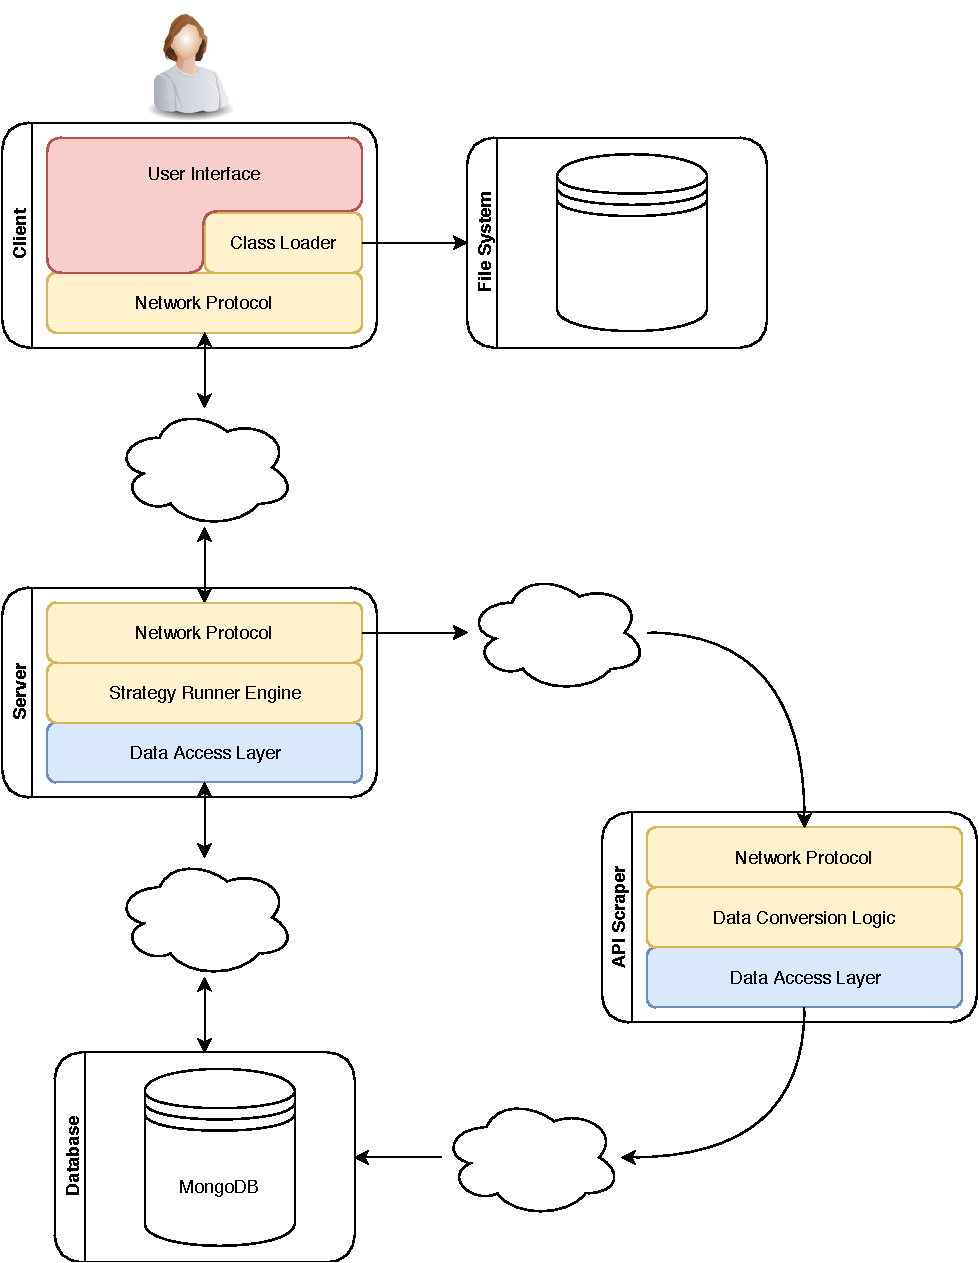
\includegraphics[width=\textwidth]{arch}
	\caption{Application architecture.}
	\label{fig:arch}
\end{figure}

\figref{fig:arch} shows the application's architecture.

\section{Third-party softwares}\label{sec:thirdparty}

The following frameworks and libraries are used:
\begin{description}
	\item[MongoDB Java Driver v3.11.2] \textit{(Server-side)} for handling
		MongoDB server;
	\item[XChart v3.6.0] \textit{(Client-side)} for chart generation;
	\item[Gson v2.8.6] \textit{(Both-side)} for JSON (de)serialization.
\end{description}

All dependencies are handled with Maven.
